\begin{solution}
    \begin{enumerate}[label = \Alph*)]
        \item I extract the first principal component of the log-returns. The time series is shown in Figure \ref{fig:pca_time_series}. This factor can explain about 5\% of the variation in the log-returns. We see that this factor picks up some volatility specially during the financial crises and the COVID-19 pandemic.
        
        \begin{figure}[!htbp]
            \begin{small}
                \begin{center}
                    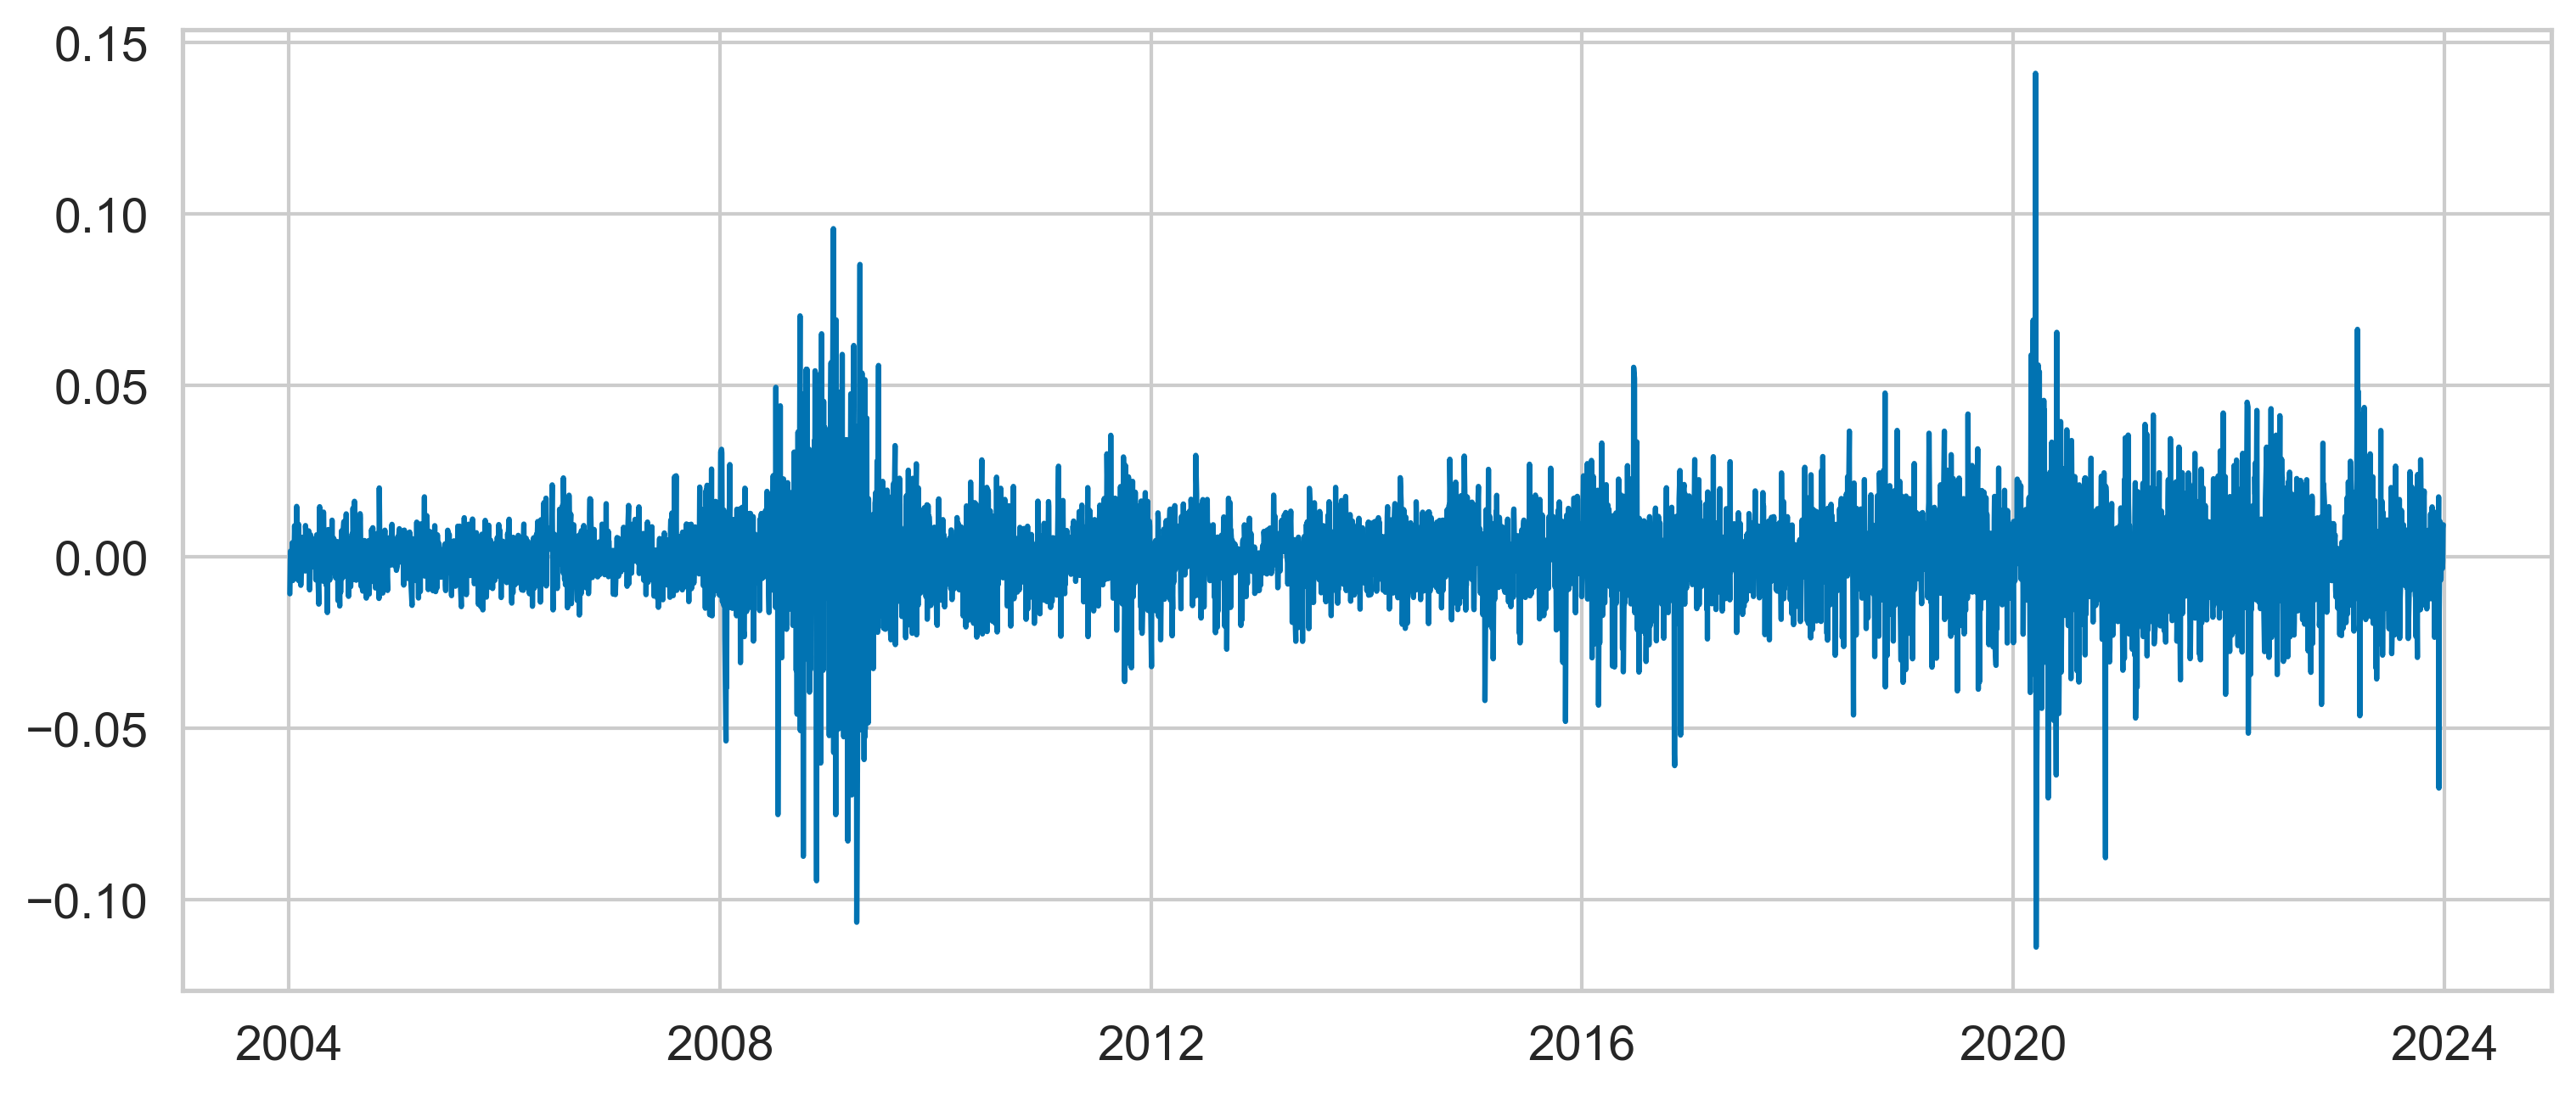
\includegraphics[width=0.95\textwidth]{pca_first_component.png}
                \end{center}
                \caption{First Principal Component of Log-Returns}
                \label{fig:pca_time_series}
            \end{small}
        \end{figure}
        
        \item I iterate the PCA analysis using 1 to 8 factors. For each one of these, I calculate the explained variance and a BIC criteria using the formula
        \begin{equation}
            \text{BIC} = T\log(\widehat\sigma_\varepsilon^2) + k \log(T)
        \end{equation}
        where \(T\) is the length of the time series, \(k\) the number of principal components and \(\widehat\sigma_\varepsilon^2\) the estimated variance of the residuals. This estimate is based on \citet{bishop2006pattern} and is available on the \texttt{scikit-learn} library. Figure~\ref{fig:pca_crit} plots the explained variable and BIC as a function of the number of factors. As we know, increasing the number of factors will always increase the explained variance. However, by penalizing it with the number of parameters estimated (using BIC), we can obtain an optimal number of factors. In this case, the BIC suggest only extracting a single factor. In contrast, the explained variance will always suggest extracting more factors.

        \begin{figure}[!htbp]
            \begin{small}
                \begin{center}
                    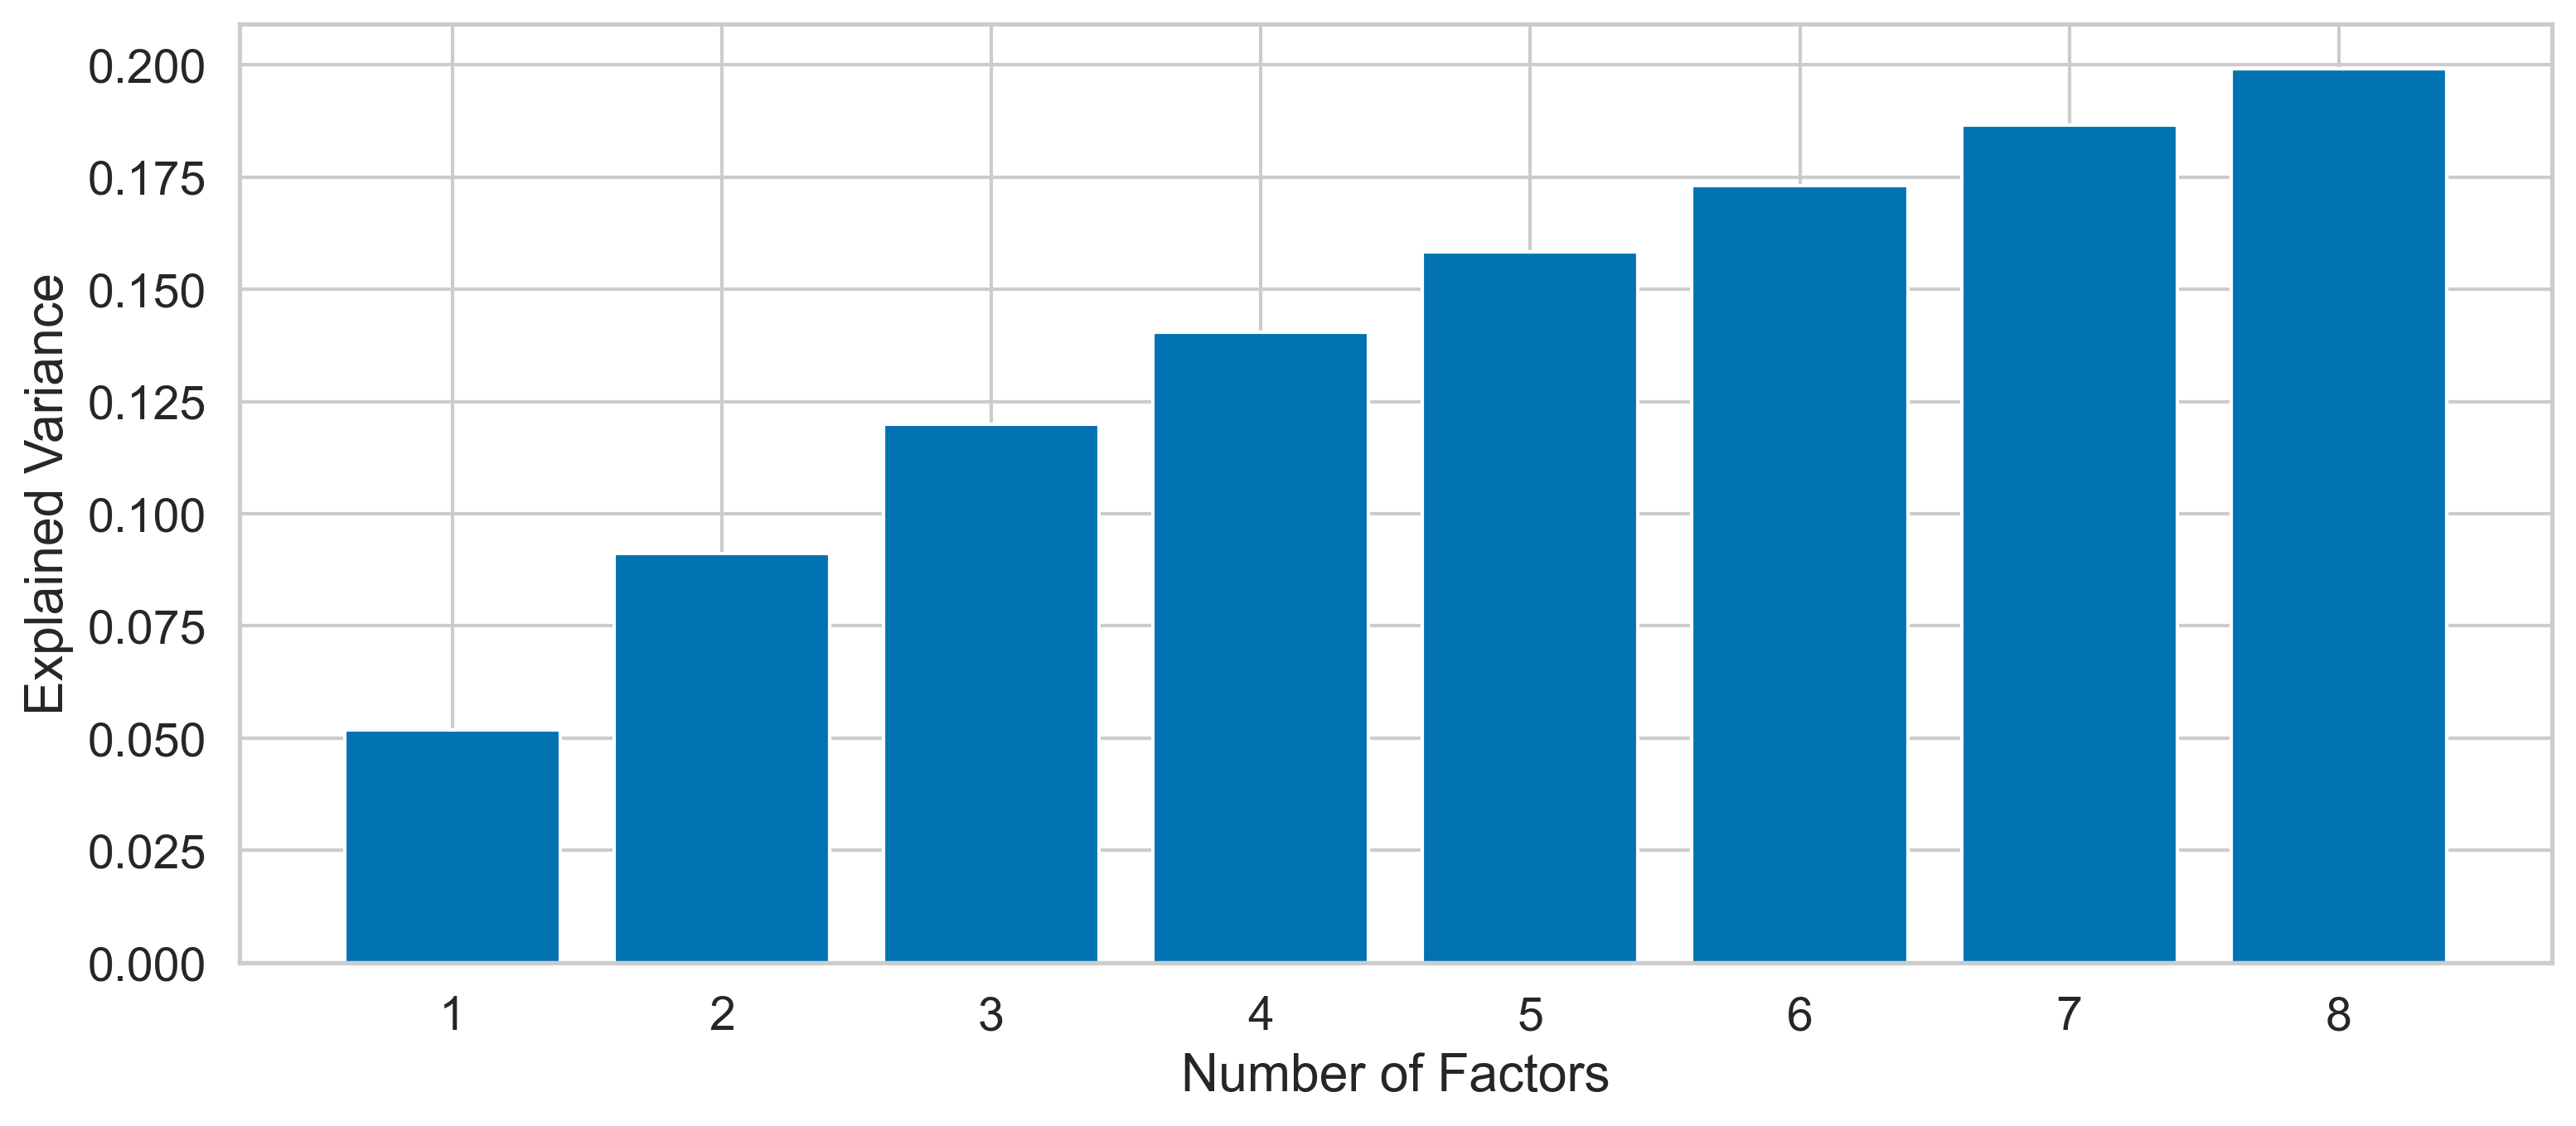
\includegraphics[width=0.95\textwidth]{pca_explained_variance.png}
                \end{center}
                \caption{Explained Variance and BIC as a Function of the Number of Factors}
                \label{fig:pca_crit}
            \end{small}
        \end{figure}
        
        \item Using the model with 8 factors, I analyze how each one of them correlate with each of the FF factors. For this, I start by showing the correlation matrix between each PCA and FF factor. This is depicted in Figure~\ref{fig:pca_ffdaily_corr}. As we can see, the first PCA factor correlates the most with the FF. PC2 tends to pick up HML as well as some Momentum.  PC4 and PC5 correlate negatively with the Market factor. PC6 seems to pick up some RMW. PC7 and PC8 don't show any significant correlation with the FF factors.
        
        \begin{figure}[!htbp]
            \begin{small}
                \begin{center}
                    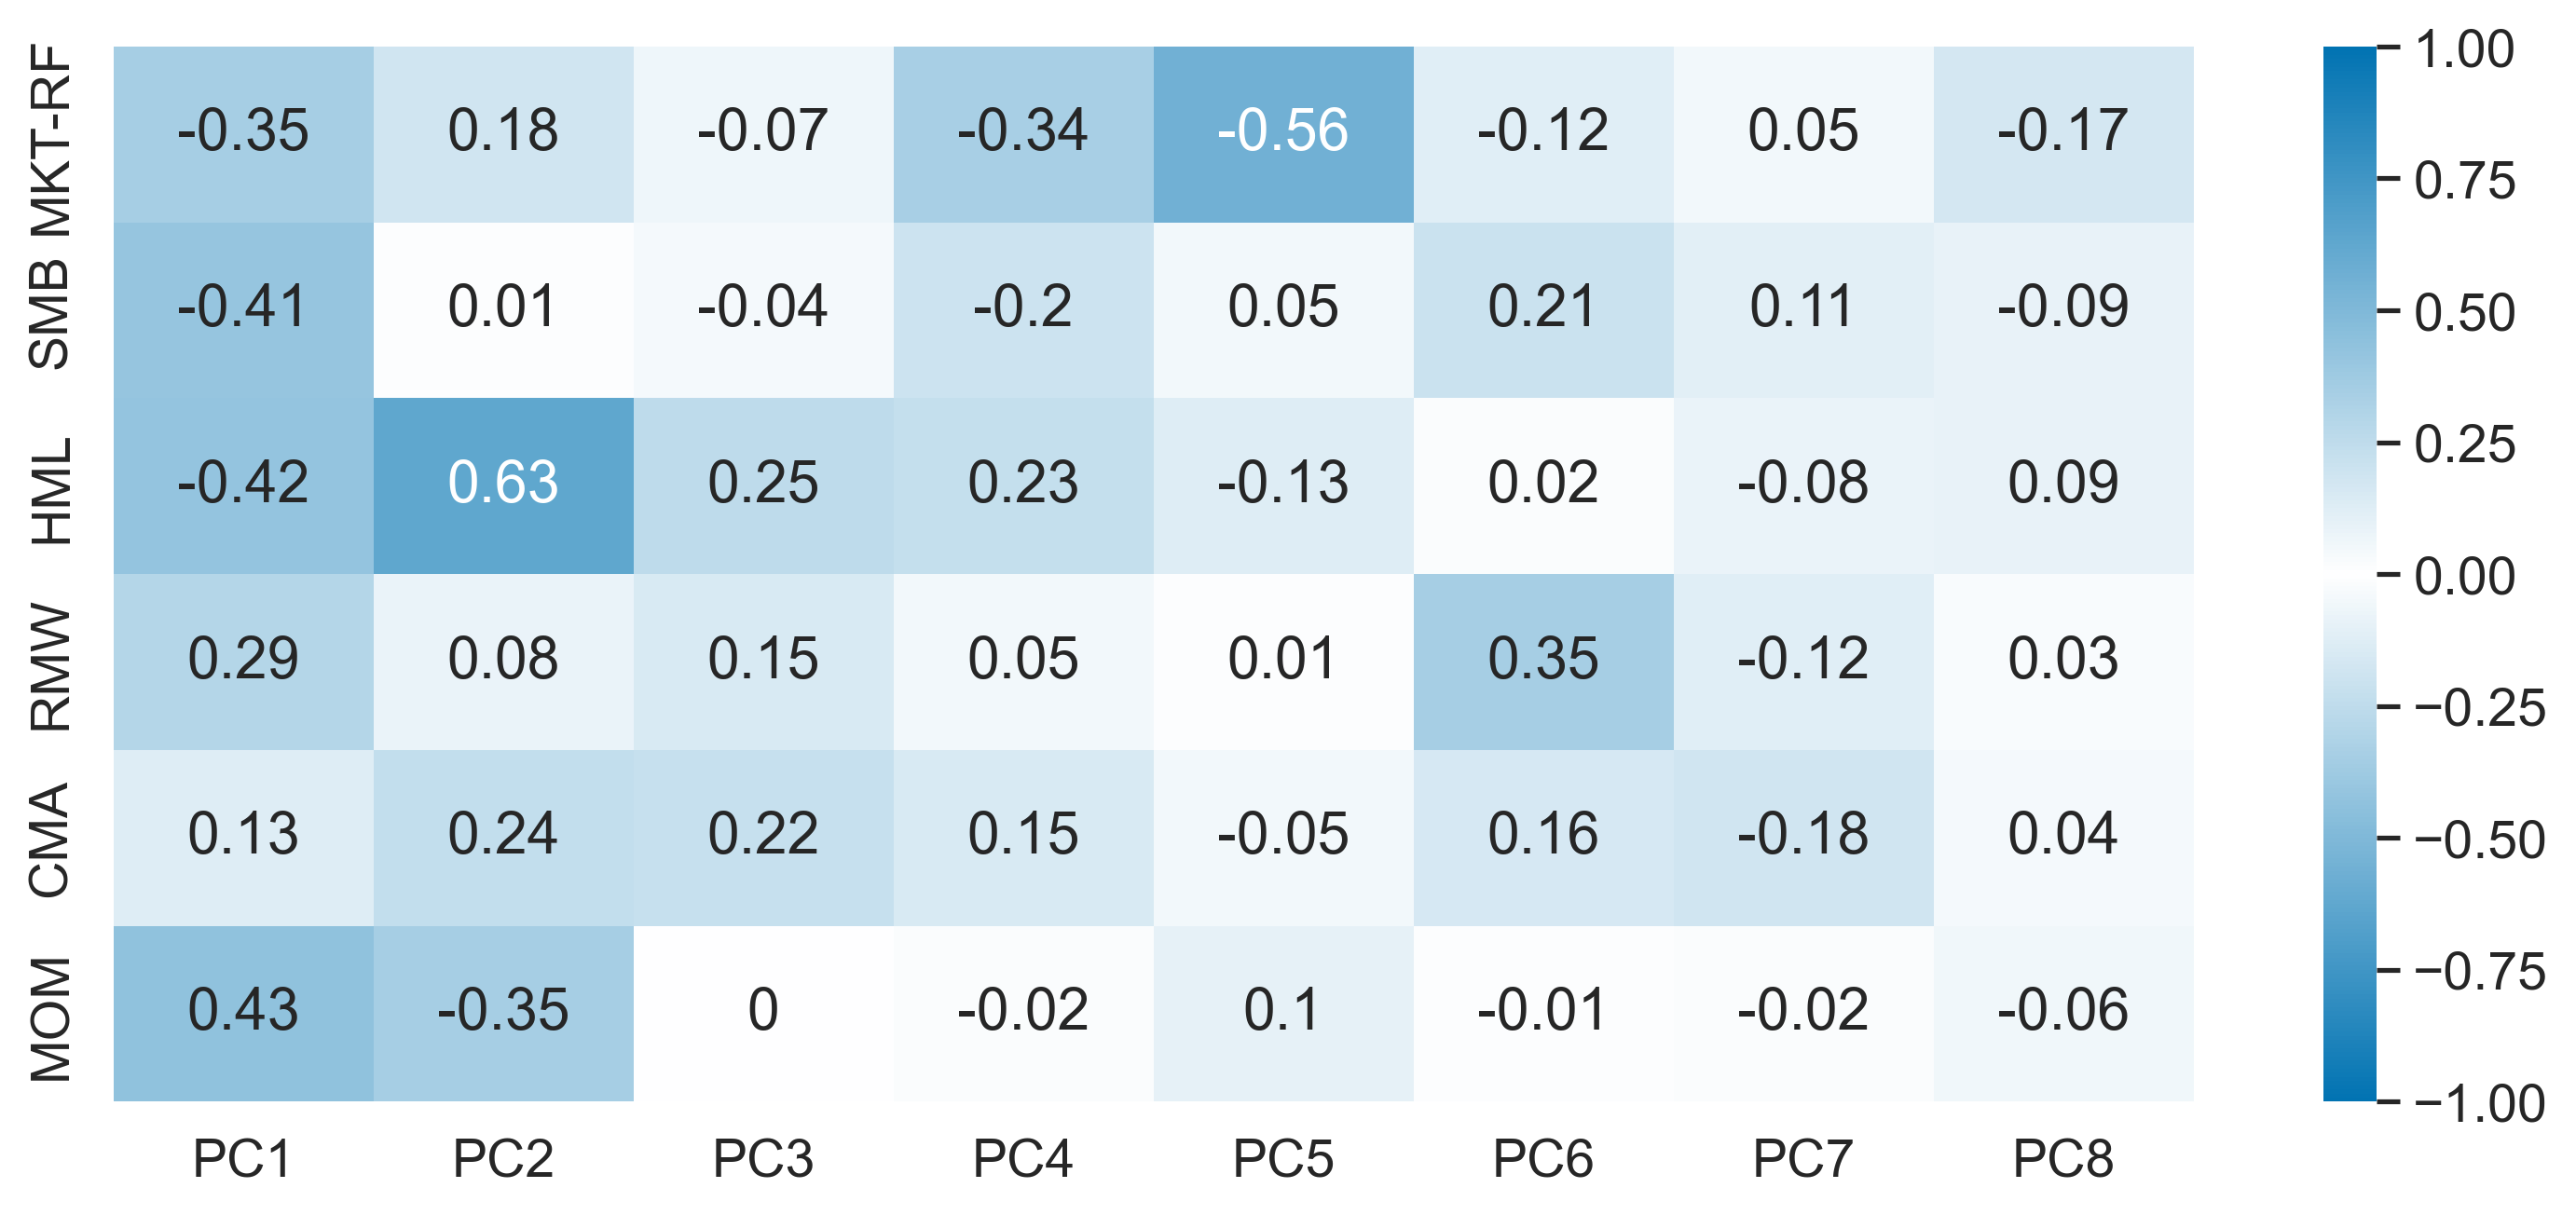
\includegraphics[width=0.95\textwidth]{pca_ffdaily_corr}
                \end{center}
                \caption{Correlation between PCA and FF factors}
                \label{fig:pca_ffdaily_corr}
            \end{small}
        \end{figure}
        
        To better understand this relationship, I run an OLS regression with each of the FF factors as a dependent variable and the PCA as the explanatory variables. This tends to capture the linear relationship between these variables. Figure~\ref{fig:pca_ffdaily_r2} shows the R-Squared of each of these regressions. According to this figure, the FF factors which mostly correlate with the PCA are Market and HML, but all of them present a significant relationship as implied by the F-test.

        \begin{figure}[!htbp]
            \begin{small}
                \begin{center}
                    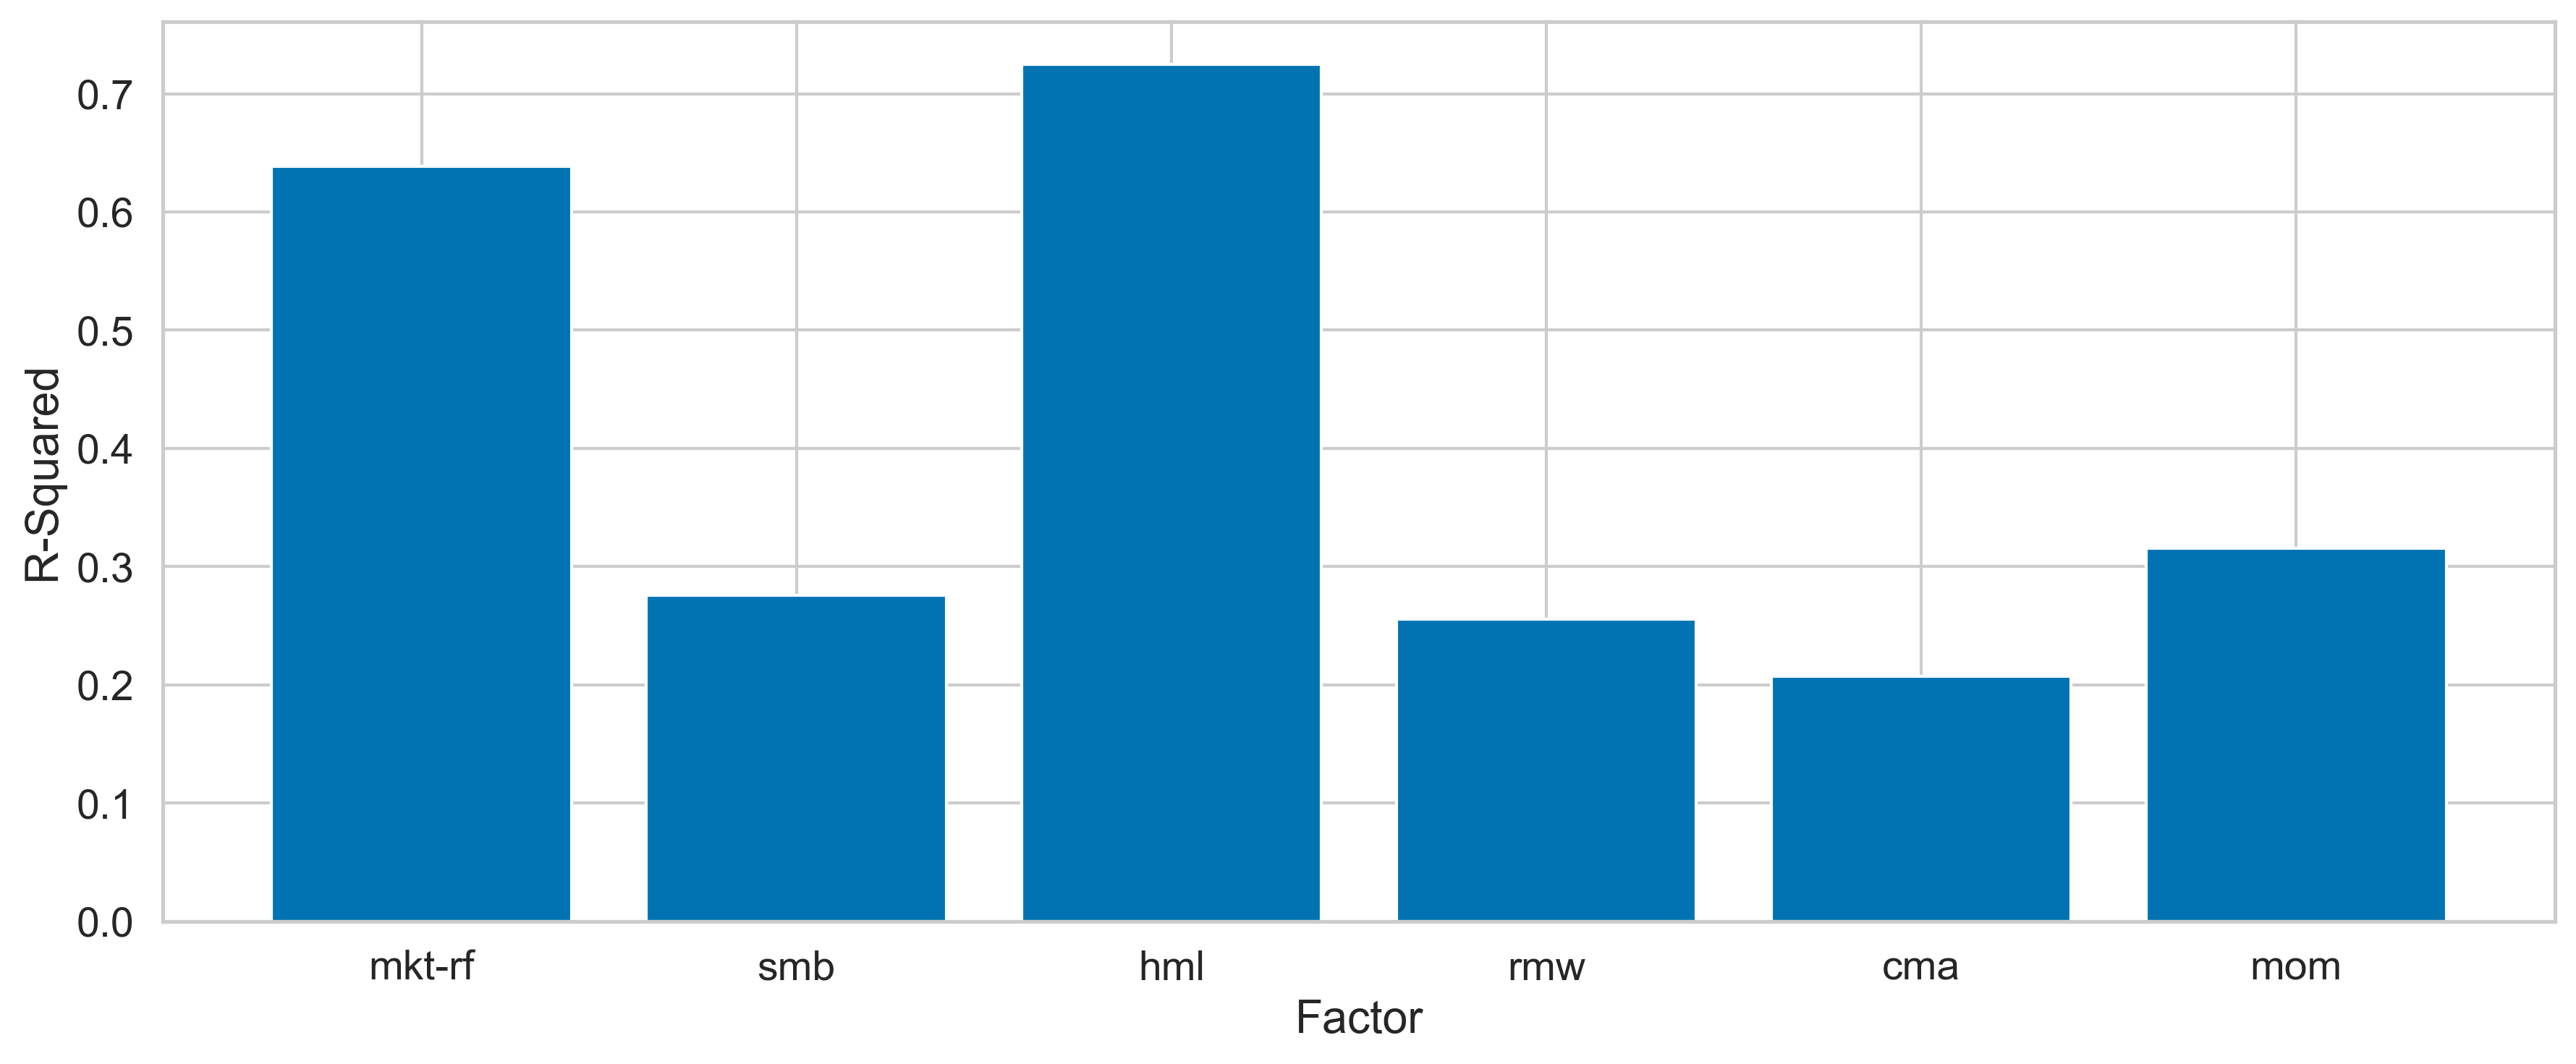
\includegraphics[width=0.95\textwidth]{pca_ffdaily_r2.png}
                \end{center}
                \caption{R-Squared of the OLS Regression between each FF factor and the Principal Components}
                \label{fig:pca_ffdaily_r2}
            \end{small}
        \end{figure}
        
        \item I now turn to the Canonical Correlation Analysis (CCA) to analyze the relationship between the FF factors and the PCA factors. I calculate the canonical correlation between these two sets of factors using 1 to 5 components. Figure~\ref{fig:cca_score} shows the canon
        ical correlation (CCA Score) as a function of the number of components. As we can see, the CCA Score starts to decrease after the inclusion of the 3rd component, suggesting an optimal number.
        
        \begin{figure}[!htbp]
            \begin{small}
                \begin{center}
                    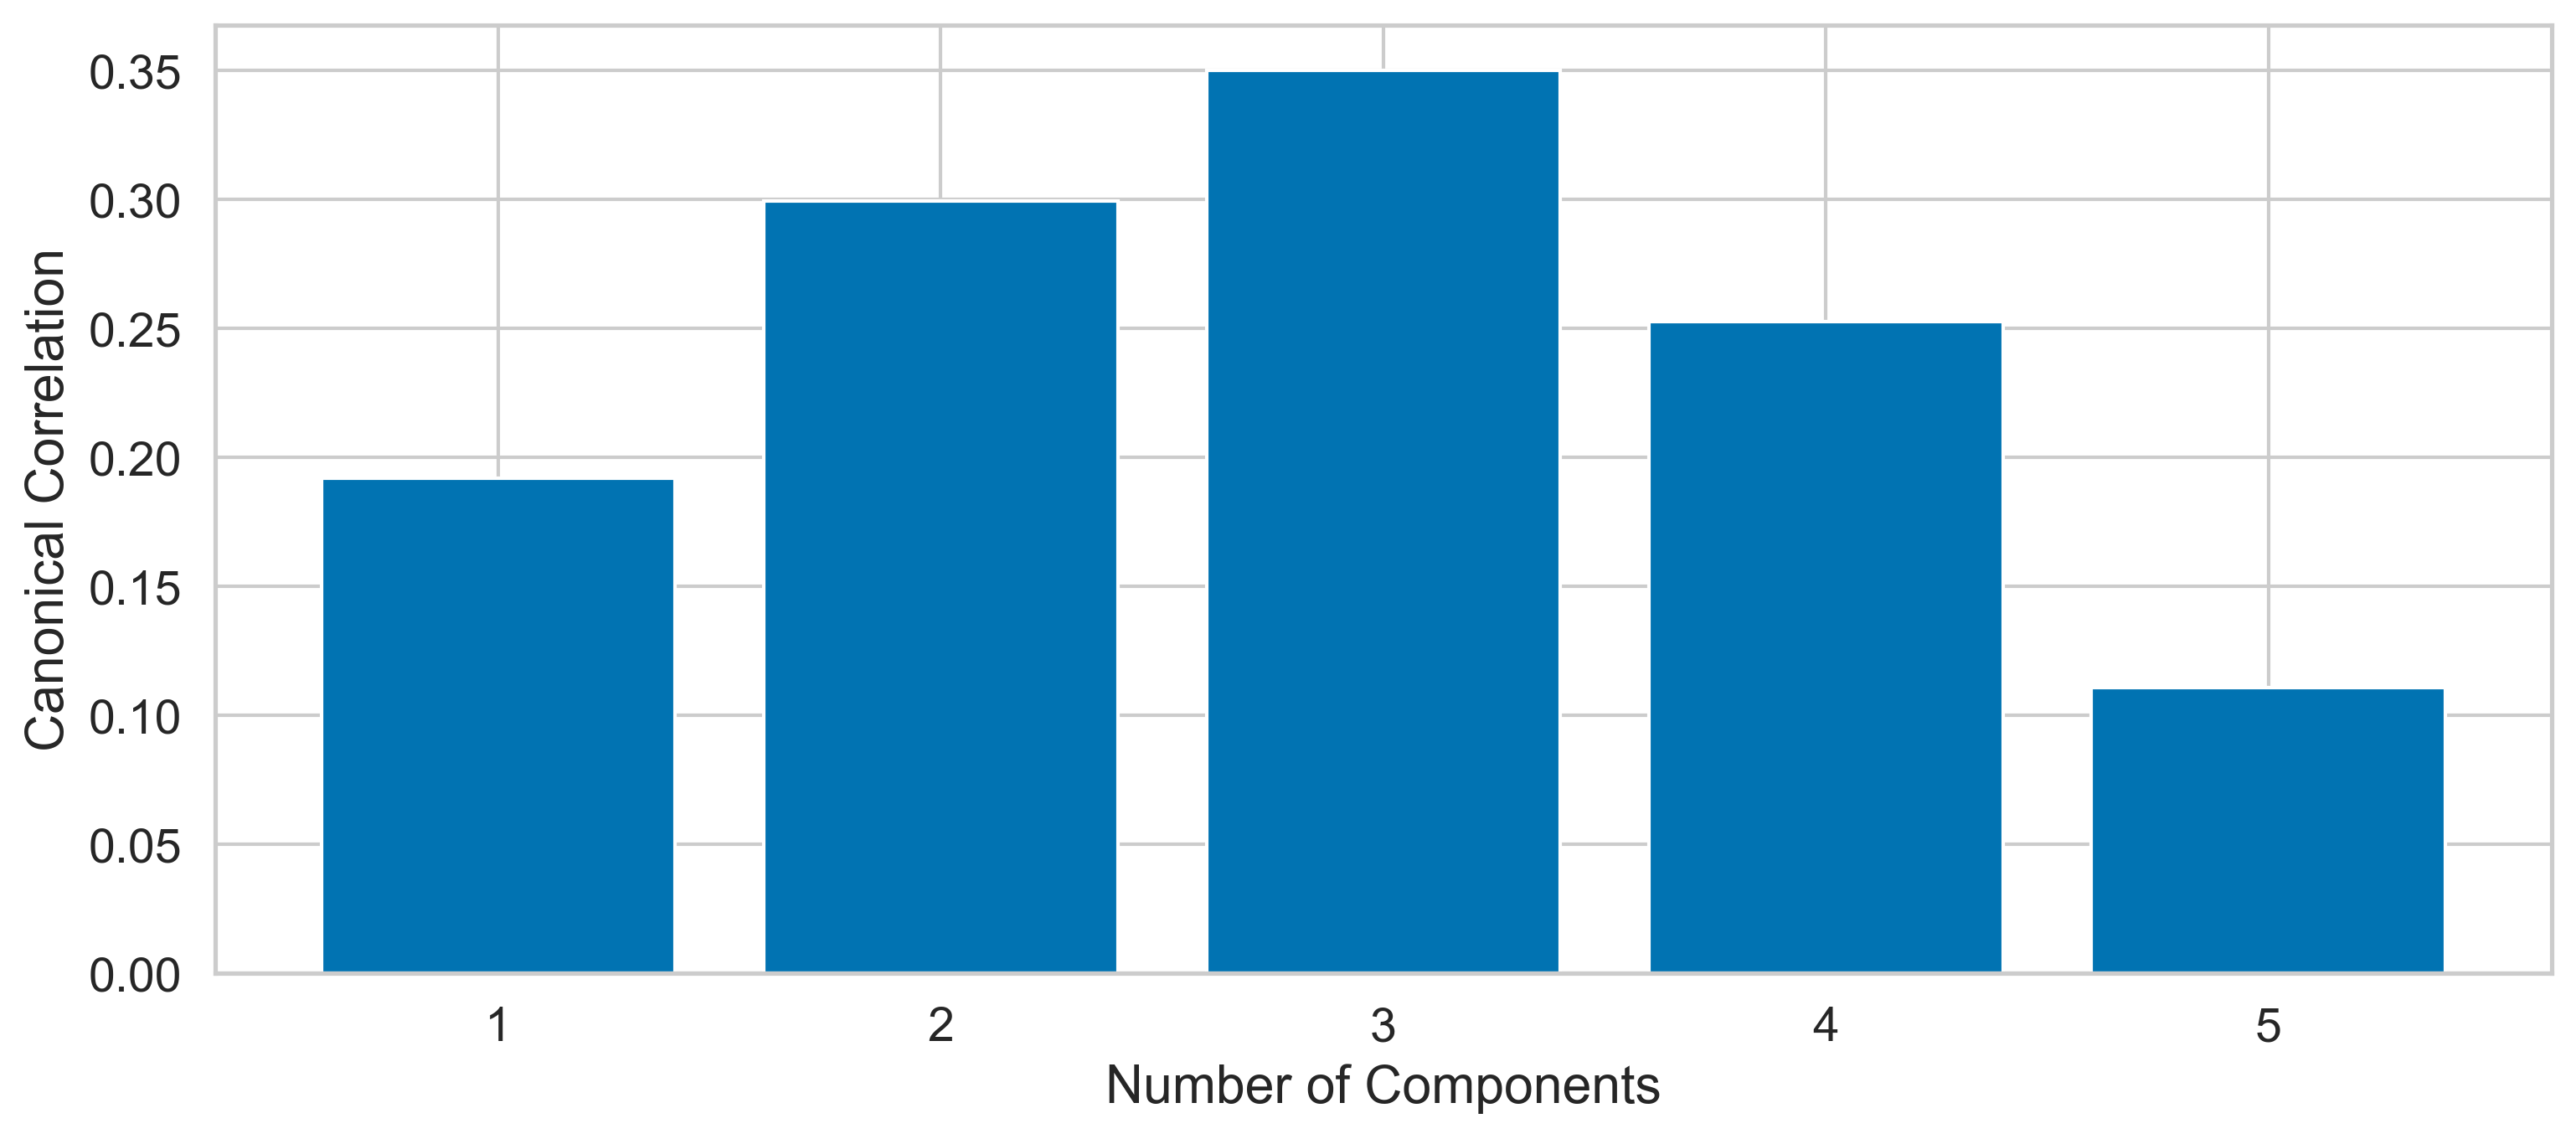
\includegraphics[width=0.95\textwidth]{cca_score}
                \end{center}
                \caption{CCA Score as a Function of the Number of Components}
                \label{fig:cca_score}
            \end{small}
        \end{figure}
        
        \item Using the model with 3 components, I rotate both the PCA and FF factors according to the CCA loadings. This helps us understand the relationship between the two set of factors. Figure~\ref{fig:canonical_variables_scatter} shows the scatter plot of each pair of canonical variables. The correlation between the first 2 pairs appears to be stronger than the 3rd. This can also be seen on the correlation matrix in Figure~\ref{fig:cca_corr}, which shows a strong correlation between the first and second pairs of canonical variables and a weaker correlation with the third pair.
        
        \begin{figure}[!htbp]
            \begin{small}
                \begin{center}
                    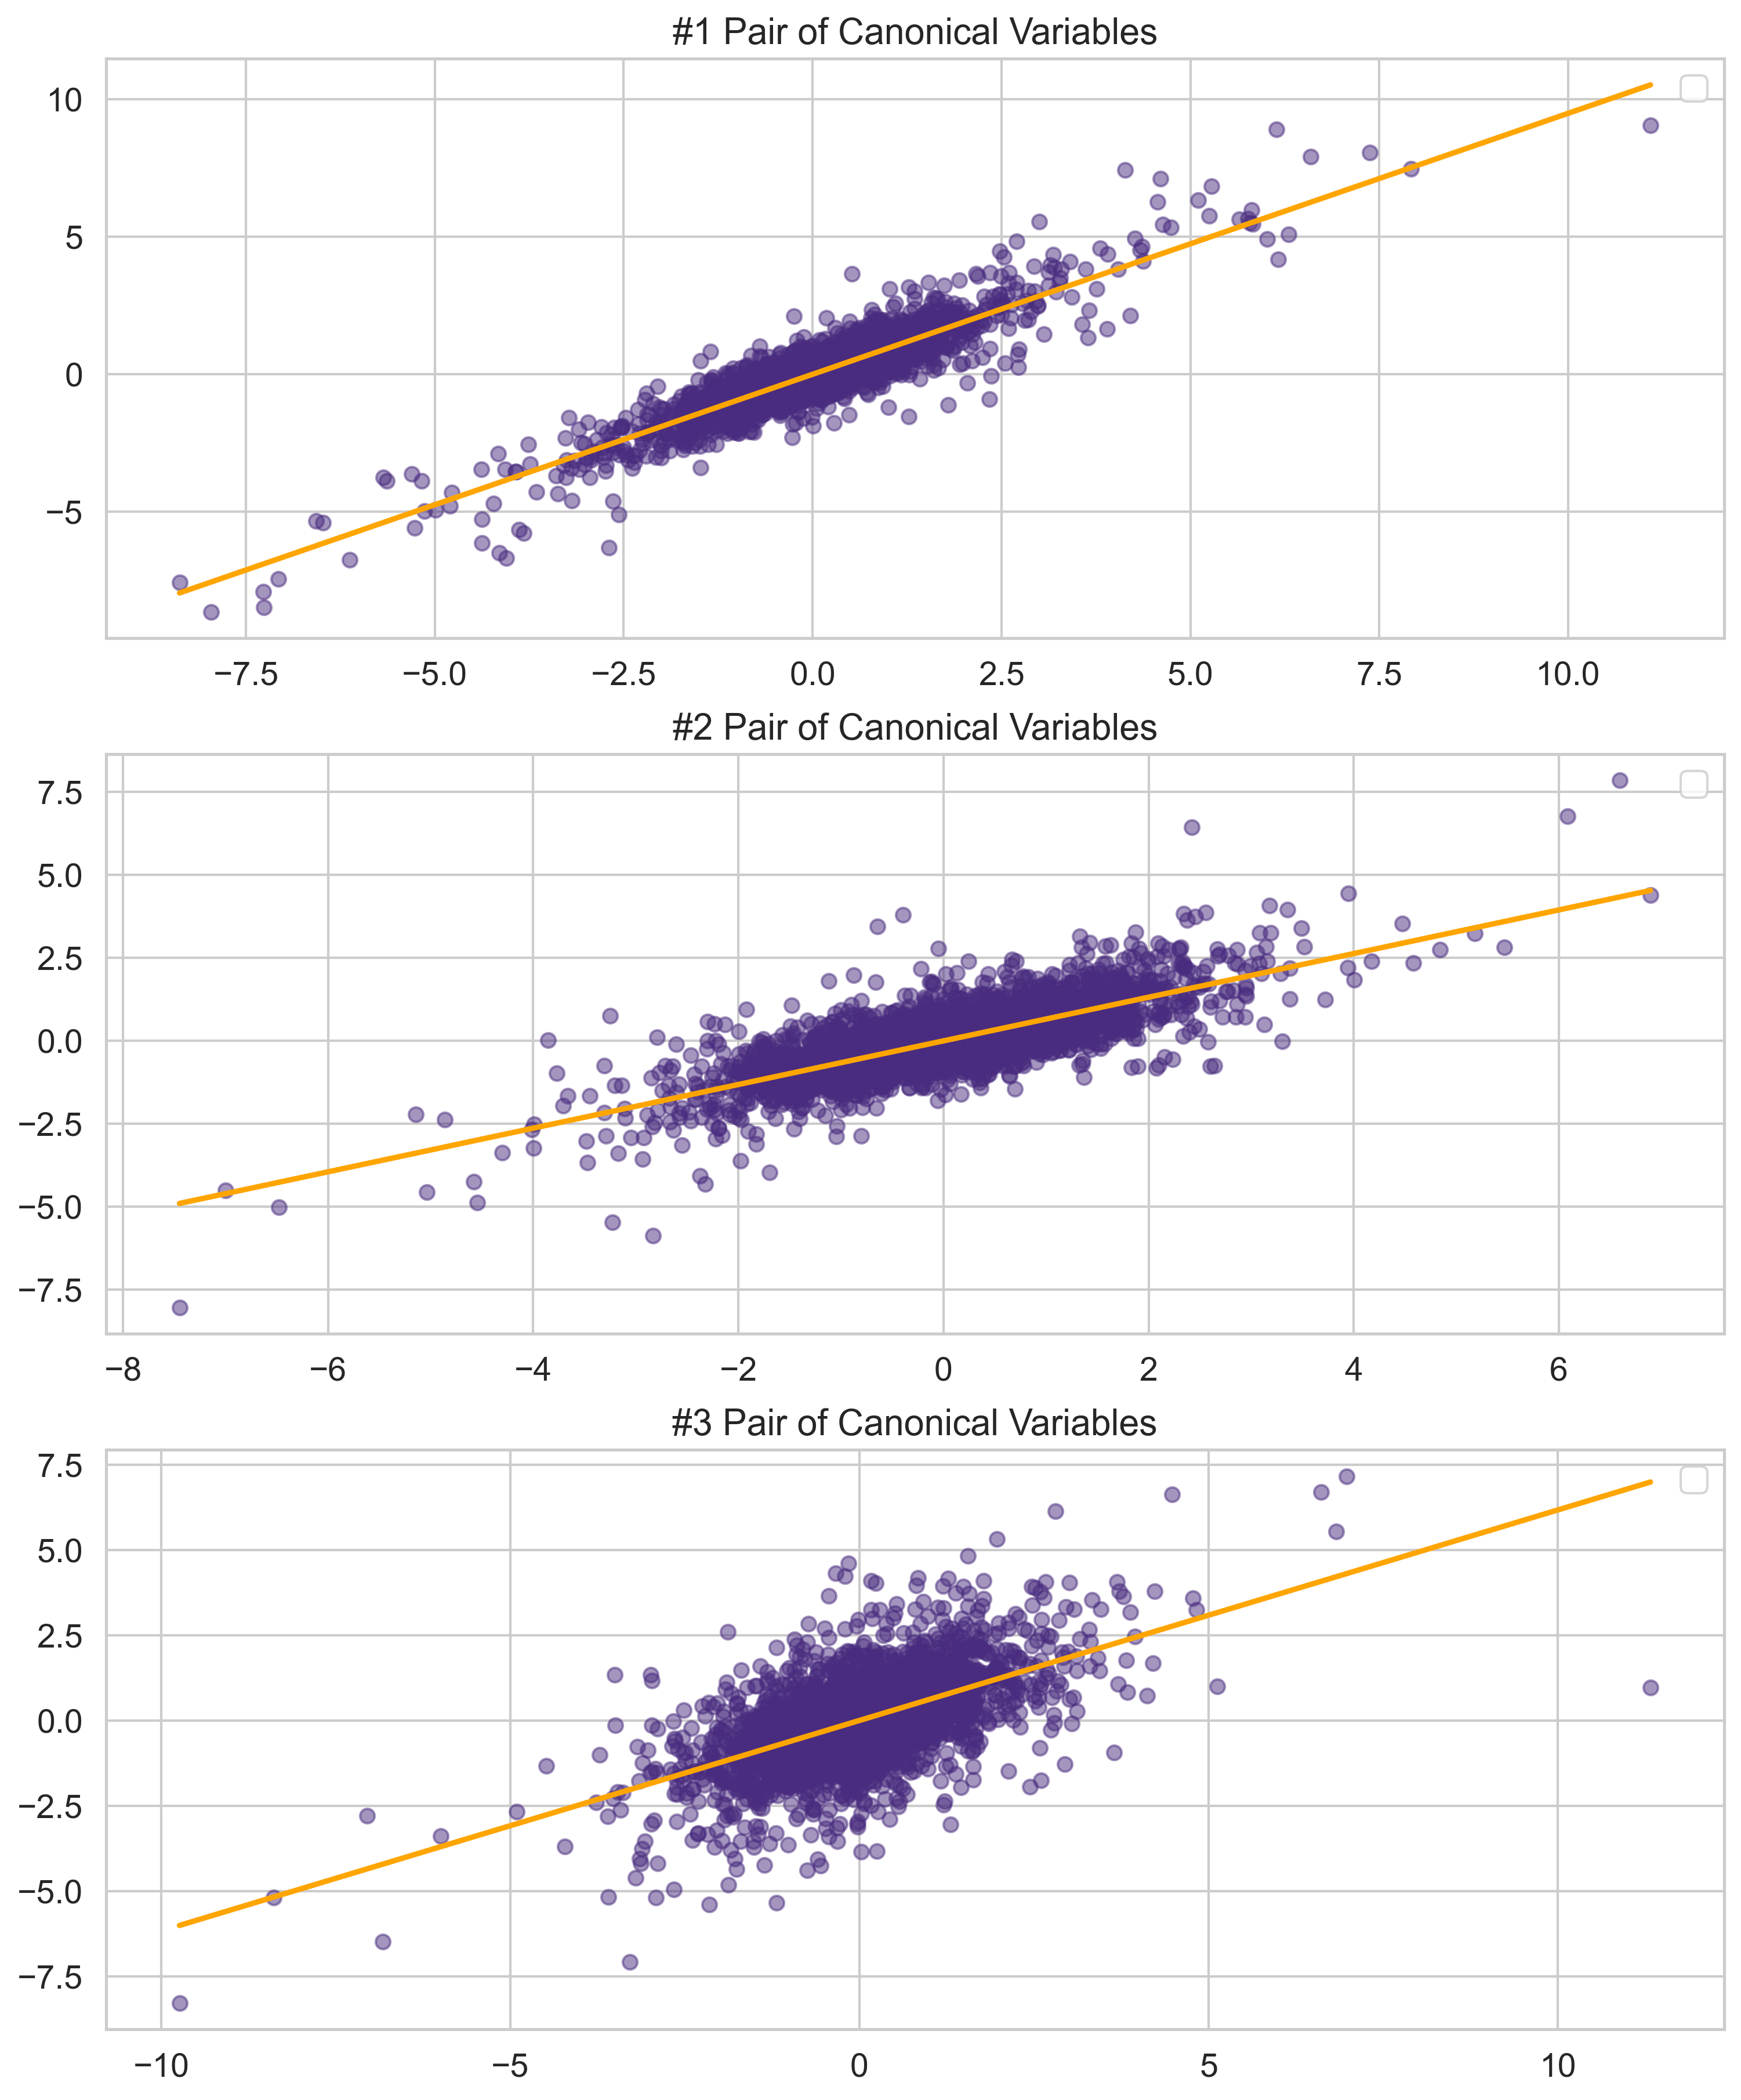
\includegraphics[width=0.95\textwidth]{canonical_variables_scatter.png}
                \end{center}
                \caption{Relationship Between Pairs of Canonical Variables}
                \label{fig:canonical_variables_scatter}
            \end{small}
        \end{figure}
        
        \begin{figure}
            \begin{small}
                \begin{center}
                    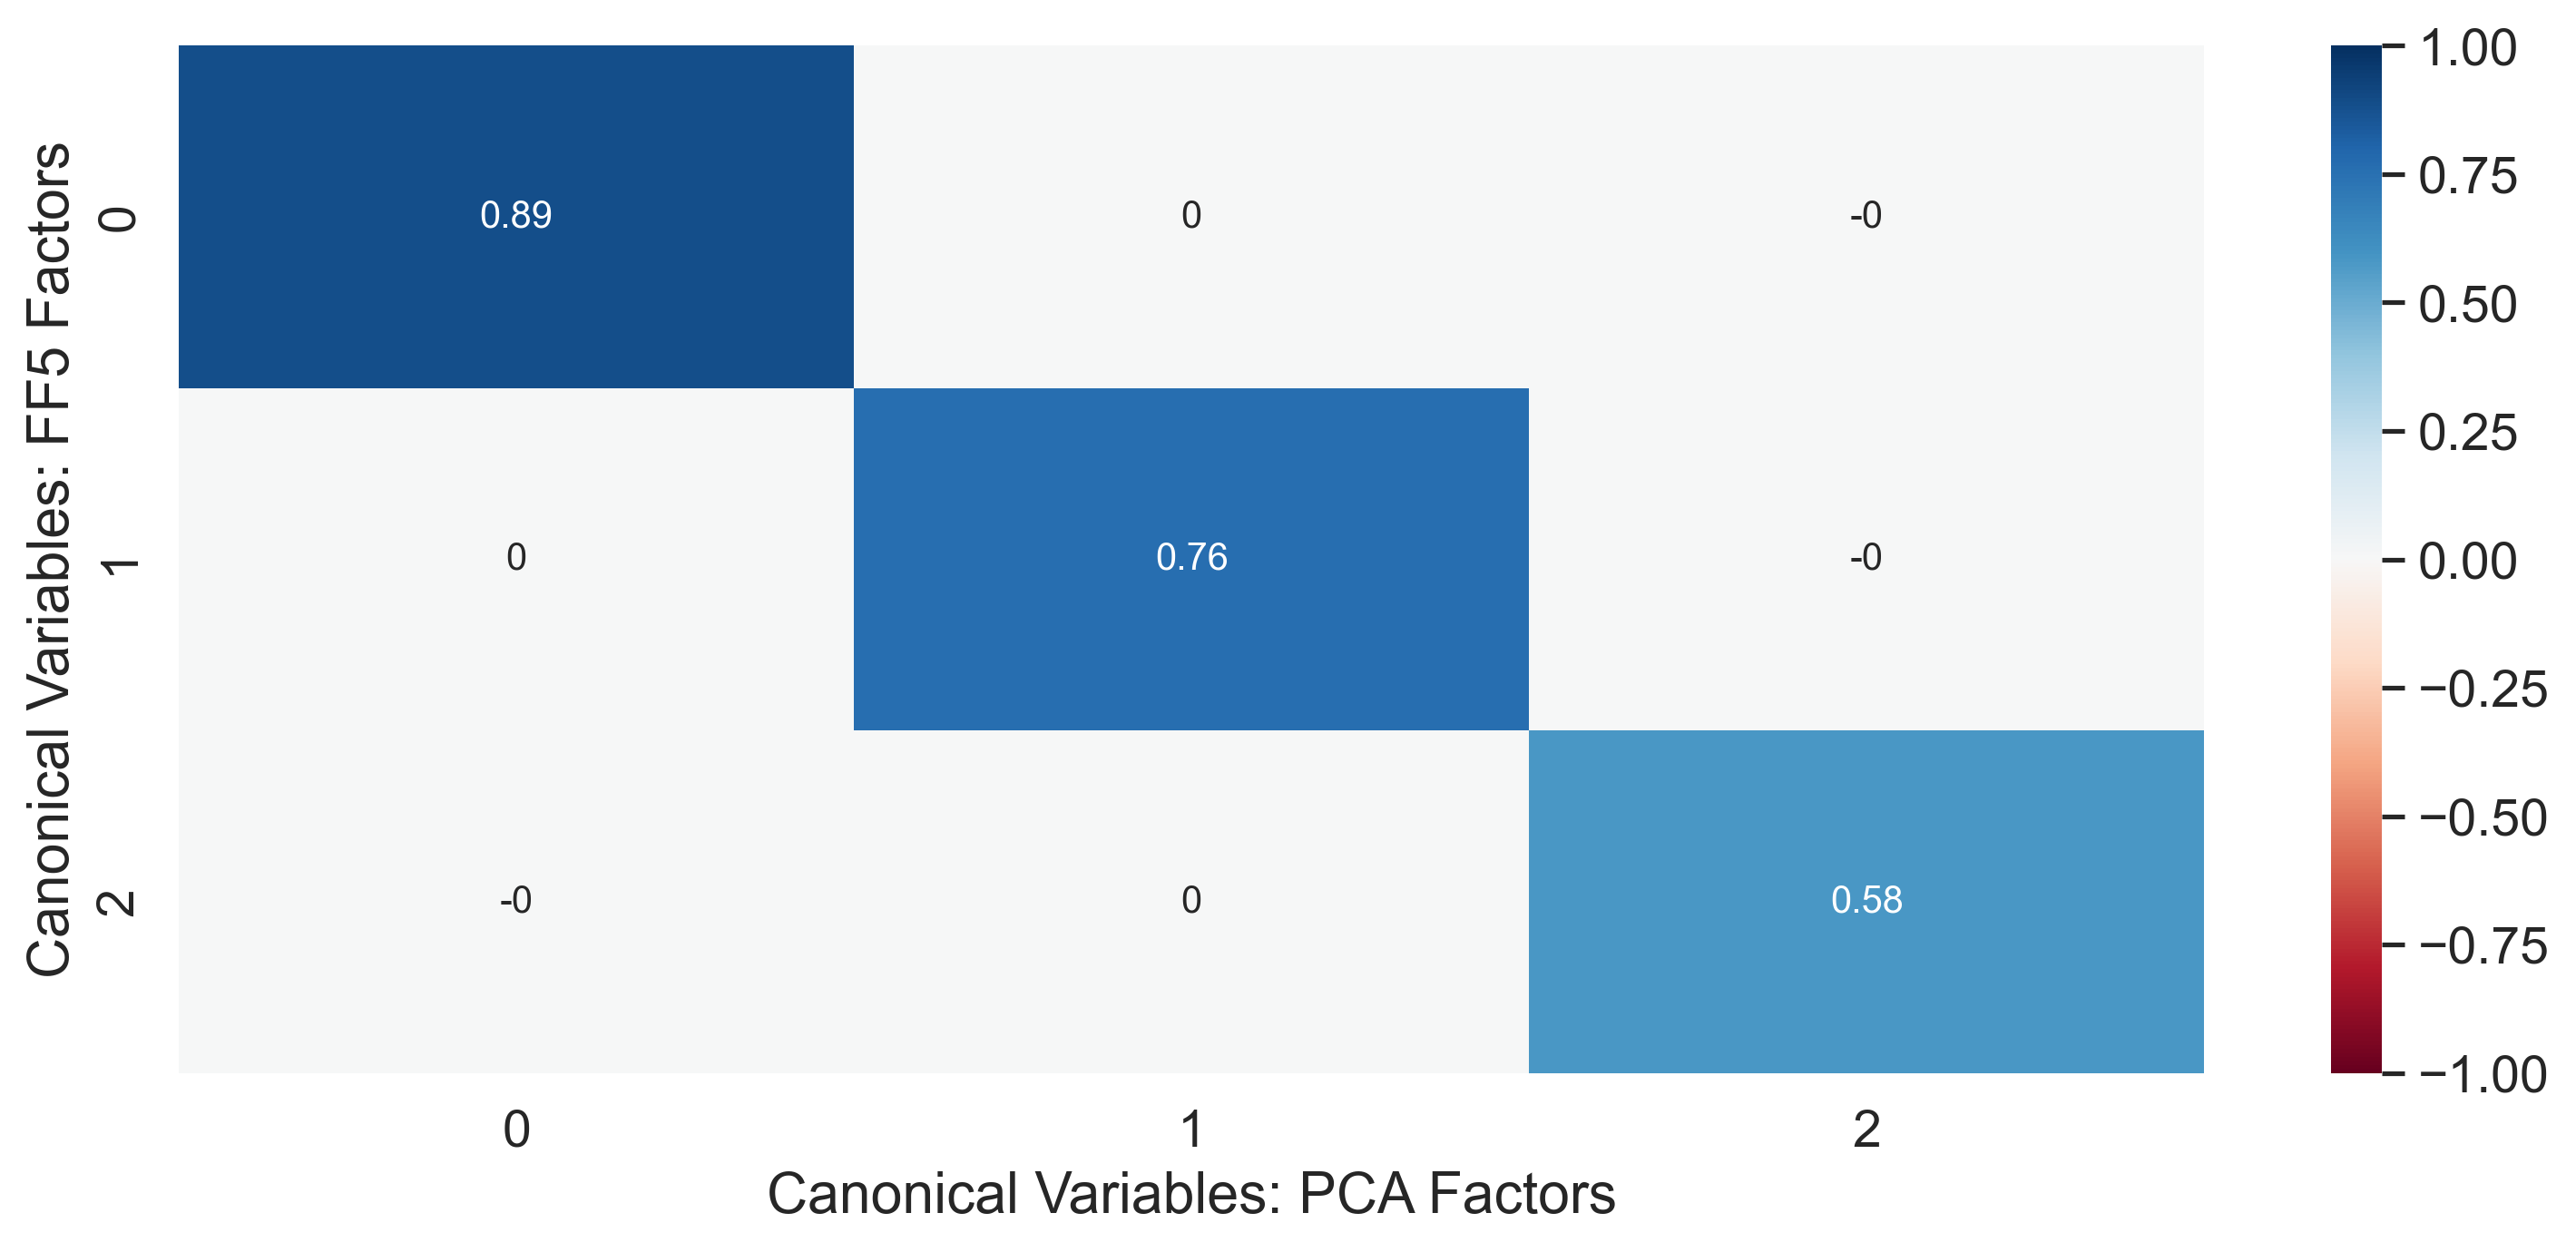
\includegraphics[width=0.95\textwidth]{cca_corr}
                \end{center}
                \caption{Correlation Between Canonical Variables}
                \label{fig:cca_corr}
            \end{small}
        \end{figure}
        
    \end{enumerate}
\end{solution}